
\section*{Schedule}

A Gannt chart detailing the duration for each task
  is shown in figure~\ref{fig:schedule}.
In this section we describe the different phases
    of the project.

We have already started the project by looking how
  easy it is to write vector add in Java such that
  it uses the same file format and timing constructs
  as Parboil.
Both vector addition and matrix multiplication have
  already been ported to Java to examine the feasibility
  of the project.
We have also already contacted the RenderScript team
  to understand what resources and services they can
  provide in terms of hardware to aid us in this project.

For the first phase of the project, we plan on porting
  4 of the simplest Parboil benchmarks to RenderScript
  (Matrix Multiply, TPACF, CUTCP, and MRI-Q).
The kernels in these benchmarks are relatively simple, 
  and most of our time would be spent setting up our 
  development environment, refining our workflow and tools, 
  and developing scripts to collect and aggregate the
  performance metrics.
The first phase ends with the first progress report where
    we plan on reporting our results for these benchmarks.


For the second phase of the project, we plan on completing
    our porting process.
There kernels in this phase are more irregular, and thus
    would be more challenging to port.
We suspect these would be the applications where low level
    control and hardware knowledge would benefit performance.
The second phase ends with the second progress report where
    we again will report the results of these benchmarks.


For the last phase of the project, we will finalize the 
    benchmarks and rerun the measurements again.
We will then, time permitting, examine what makes RenderScript
    either efficient or inefficient and what runtime and/or
    compiler optimizations can be performed to either 
    increase performance or increase programmability.
Based on this we will modify our kernels to make use of these
    learned insights and report the performance in the final
    report.

\begin{figure}[t!]
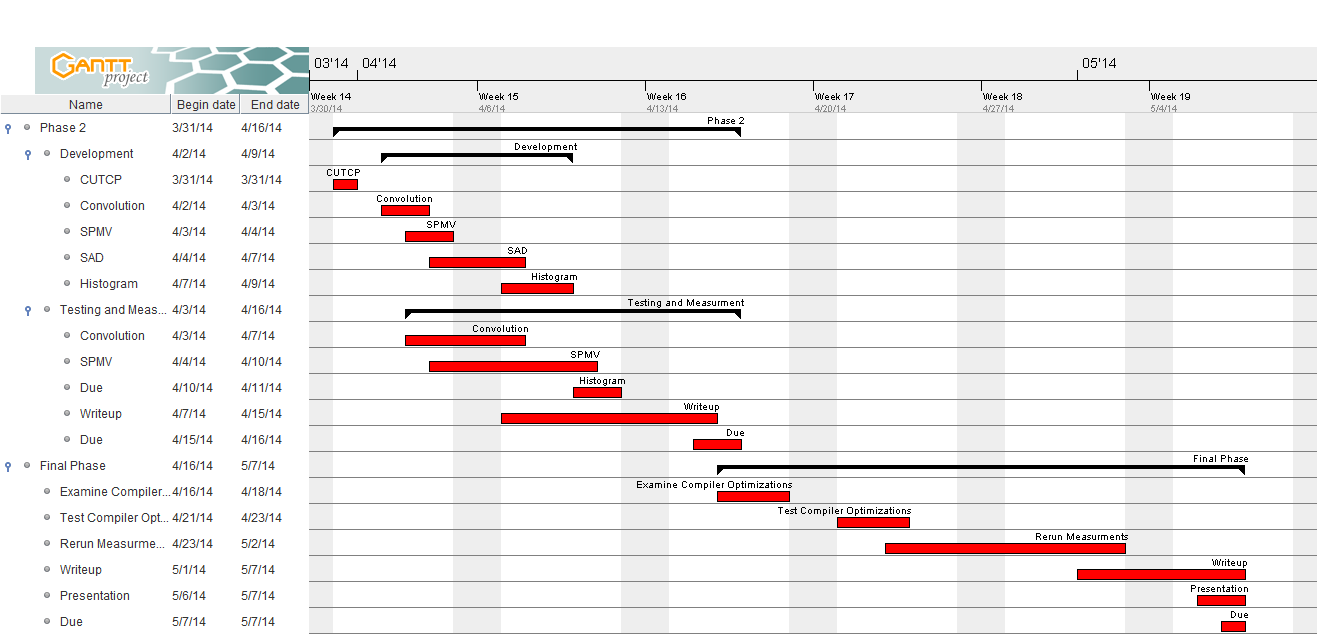
\includegraphics[scale=0.16, angle=90]{chart.png}
\caption{Projected project schedule.}
\label{fig:schedule}
\centering
\end{figure}
